\chapter{能量與哈密頓量}

\lectureoverview{我們先進一步釐清主動對稱性的意義，並回顧平移與旋轉如何對應到動量和角動量的守恆。尚未導出的守恆量是能量；對應的對稱性是時間平移，而守恆量是哈密頓量\(H=\sum_i p_i\dot q_i-L\)。推導也會精確說明，顯式時間依賴如何使能量在選定的子系統與其環境之間傳遞。}

\section{正式論證前的問題}

我們即將達到後續主題所需的經典力學最低限度，不過力學中仍有許多值得學習的內容。開始主要論證之前，曾有兩個問題提出。

\begin{classroomqa}
  \audiencequestion{這門入門課程之後，有哪些值得參考的書？
  \lecturetimestamp{00:00:36--00:02:13}}
  \lecturerresponse{公認的進階參考書是 Herbert
  Goldstein 的 \emph{Classical Mechanics}。Cornelius Lanczos 關於力學變分原理的著作也是相關參考資料。提供一份課堂閱讀書單，比假定一位講師能概覽所有可用教材更實際。}
\end{classroomqa}

第二個問題記錄了當時一項尚未解決的測量結果。在 2011 年，OPERA 實驗曾報告，從 CERN 傳送至 Gran Sasso 的中微子似乎提早抵達。所報告的時間差比產生中微子所用的質子脈衝還短，因此時間分析必須比較脈衝輪廓，而無法在發射時標記某一個中微子，再於探測時辨認出同一個粒子。

\begin{classroomqa}
  \audiencequestion{中微子表觀超光速的結果後來解決了嗎？
  \lecturetimestamp{00:02:30--00:09:03}}
  \lecturerresponse{當時還不能下結論。束流脈衝形狀、靶材受熱與同步問題都需要仔細檢視。一項推測性的提議考慮了 GPS 衛星的運動：在衛星參考系中，源與探測器都在移動，而定時訊號也在傳播，因此會產生數十奈秒量級的修正。這項估算作為數量級的練習很有意思，但當時並未將它視為對該實驗可信的診斷。在相關速度下，通常的洛倫茲收縮效應太小，無法解釋所報告的差異。適當的做法是等待實驗分析結果。}
\end{classroomqa}

\begin{figure}[htbp]
  \centering
  \includegraphics[width=0.78\textwidth]{lecture_05_figure_07.png}
  \caption{討論歷史上的中微子測量問題時提到的衛星參考系定時示意圖。}
  \lectureframe{00:06:30}
\end{figure}

以下力學討論用不到這段定時問題。不過，它仍提醒我們：看似合理的尺度估算，並不等於已確立的實驗解釋。

\section{主動對稱性與系統的選取}

讓我們回到前面討論得還不夠清楚的問題：對稱性究竟是什麼？考慮直線上的一個粒子，以及以下指令：
\begin{equation}
  x\longrightarrow x+1.
  \label{eq:l5-shift-one}
\end{equation}
這個指令有兩種理解方式。\emph{被動}變換會重新標記直線上的各點。原本稱為\(x=0\)的點，現在可以改稱\(x'=1\)，但粒子本身並未移動。\emph{主動}變換則保持標籤不變，直接將粒子從\(x\)移至\(x+1\)。只有第二種操作會改變粒子相對於外部勢的位置。

\begin{figure}[htbp]
  \centering
  \includegraphics[width=0.82\textwidth]{lecture_05_figure_08.png}
  \caption{規則\(x\mapsto x+1\)、固定不變的座標軸，以及外部勢，三者共同區分主動運動與被動重新標記。}
  \lectureframe{00:11:20}
\end{figure}

\begin{classroomqa}
  \audiencequestion{若移動粒子會改變其勢能，是否表示勢的來源被排除在系統之外？
  \lecturetimestamp{00:12:19--00:14:18}}
  \lecturerresponse{正是如此。把系統稱為``處於勢中的粒子''，就是把世界分成粒子與產生\(V(x)\)的重質環境，例如地球。地球確實會反衝，但在此近似下，地球的質量極大，反衝效應可以忽略。相對於固定的地球移動粒子，會改變\(V\)；若將粒子與地球一起平移，則不會改變。}
\end{classroomqa}

\begin{classroomqa}
  \audiencequestion{在先前的旋轉例子中，速度也和位置一樣改變了嗎？
  \lecturetimestamp{00:14:26--00:15:29}}
  \lecturerresponse{是的。剛性的主動旋轉作用於整段運動歷程，而不只是某一瞬間的位置；位置向量與速度向量都會旋轉。相較之下，若在每個時刻都施加相同的平移，\(x\)會改變，但\(\dot x\)保持不變。}
\end{classroomqa}

系統與環境的區分還會再次出現兩次：一次是在含時裝置與子系統交換能量時，另一次是在宏觀摩擦使能量隱藏於未觀測到的微觀運動中時。

\section{組態空間中的無窮小位移}

一般力學系統的組態，是廣義座標\(q_i\)空間中的一個點。主動無窮小變換會將每一個可能的組態移至鄰近位置。我們寫成
\begin{equation}
  \delta q_i=\epsilon f_i(q),
  \label{eq:l5-general-transformation}
\end{equation}
其中函數\(f_i\)定義了組態空間上的一個固定位移場。它們可以依賴所有座標，其中某些函數也可能為零。共同因子\(\epsilon\)很小，用來將步長的大小與變換的形式分開。

\begin{figure}[htbp]
  \centering
  \includegraphics[width=0.75\textwidth]{lecture_05_figure_09.png}
  \caption{組態空間中每一點上所附的位移向量。}
  \lectureframe{00:16:50}
\end{figure}

\begin{figure}[htbp]
  \centering
  \includegraphics[width=0.80\textwidth]{lecture_05_figure_10.png}
  \caption{依賴座標的無窮小變換
  \(\delta q_i=\epsilon f_i(q)\)。}
  \lectureframe{00:18:00}
\end{figure}

變換規則本身沒有顯式時間依賴，因此它對速度的作用為
\begin{equation}
  \delta\dot q_i=\frac{d}{dt}(\delta q_i)
  =\epsilon\sum_j\frac{\partial f_i}{\partial q_j}\dot q_j.
  \label{eq:l5-velocity-variation}
\end{equation}
對平移而言，\(f_x=1\)，因此\(\delta\dot x=0\)。對旋轉而言，\(f_i\)依賴位置，所以速度也會改變。

\begin{classroomqa}
  \audiencequestion{在
  \(\delta q_i=\epsilon f_i(q)\)中，最後那個小因子在每一點都是相同的常數嗎？
  \lecturetimestamp{00:19:58--00:20:51}}
  \lecturerresponse{是的。單一常數\(\epsilon\)只是記號上的安排，讓所有座標變化都以同一個小量作為一階量。空間依賴性包含在函數\(f_i(q)\)中，而不在\(\epsilon\)中；這些函數本身不必很小。}
\end{classroomqa}

\section{變換在什麼條件下才是對稱性？}

主動變換通常會改變勢能，也可能改變動能。在曲線座標中，動能項的形式為
\begin{equation}
  T=\frac12\sum_{i,j}g_{ij}(q)\dot q_i\dot q_j,
  \label{eq:l5-kinetic-metric}
\end{equation}
因此，在組態空間中移動可能會改變其係數。極座標中熟悉的\(r^2\dot\theta^2\)項，就是最簡單的例子。

在此，若\emph{整個}拉格朗日量的一階變化為零，這個變換便是對稱性：
\begin{equation}
  \delta L=O(\epsilon^2),
  \label{eq:l5-symmetry-condition}
\end{equation}
而且這個條件必須在組態空間的每一點都成立，不能只在某個特定解所經過的組態成立。

例如，在\(x\mapsto x+\epsilon\)下，
\begin{equation}
  \delta V=\frac{\partial V}{\partial x}\epsilon.
  \label{eq:l5-potential-variation}
\end{equation}
若對每個可能的\(x\)而言，此變化都為零，則\(\partial V/\partial x=0\)：勢能不依賴\(x\)。若勢能在沿所有空間方向的平移下都不變，它就是常數。

\begin{figure}[htbp]
  \centering
  \includegraphics[width=0.80\textwidth]{lecture_05_figure_11.png}
  \caption{沿\(x\)方向的平移，以不依賴\(x\)的勢能\(V(y)\)作為檢驗對象。}
  \lectureframe{00:23:40}
\end{figure}

對於光滑的單參數變換族，只要一階變化在每一點都為零，就能將無窮小步驟接續起來，得到有限變換下的對稱性。

\begin{classroomqa}
  \audiencequestion{動能與勢能必須分別保持不變嗎？
  \lecturetimestamp{00:24:44--00:25:33}}
  \lecturerresponse{不必。只要求總拉格朗日量保持不變。有些拉格朗日量含有座標--與速度的混合項，無法有意義地分成\(T\)和\(V\)；在這種情況下，要求兩者分別不變甚至可能沒有意義。}
\end{classroomqa}

\begin{classroomqa}
  \audiencequestion{``沒有變化''是指完全沒有變化，還是指變化小到可以忽略？
  \lecturetimestamp{00:25:34--00:28:59}}
  \lecturerresponse{對無窮小變換而言，意思是沒有與\(\epsilon\)成正比的項。在局部計算中，會略去\(\epsilon^2\)階的項。由於一階條件沿單參數軌道處處成立，反覆施行局部步驟便得到有限變換下的不變性。}
\end{classroomqa}

\section{重新導出動量與角動量}

對於此處考慮的精確、定時不變的點變換對稱性，先前證明的結果為
\begin{equation}
  Q=\sum_i p_i f_i(q),
  \qquad
  p_i=\frac{\partial L}{\partial\dot q_i},
  \qquad
  \dot Q=0.
  \label{eq:l5-noether-charge}
\end{equation}
因子\(\epsilon\)不包含在\(Q\)中；它只表示我們沿對稱性軌道移動的幅度。

\begin{figure}[htbp]
  \centering
  \includegraphics[width=0.82\textwidth]{lecture_05_figure_12.png}
  \caption{一般無窮小位移及其對應的諾特守恆量。}
  \lectureframe{00:30:00}
\end{figure}

沿\(x\)方向平移時，\(f_x=1\)，且\(Q=p_x\)。若平移對稱性涵蓋所有方向，動量的三個分量都守恆。對多個相互作用的粒子而言，這種對稱性會將所有粒子一起平移；若相互作用只依賴相對位置，則\begin{equation}
  \mathbf P=\sum_a\mathbf p_a
  \label{eq:l5-total-momentum}
\end{equation}守恆。只移動某一粒子，使它相對於其餘粒子位移，並不屬於這種對稱變換。

\begin{figure}[htbp]
  \centering
  \includegraphics[width=0.80\textwidth]{lecture_05_figure_13.png}
  \caption{共同平移使總動量的各分量分別守恆。}
  \lectureframe{00:32:50}
\end{figure}

在\(x\)-\(y\)平面內作無窮小旋轉時，選取以下旋轉方向：
\begin{equation}
  \delta x=-y\epsilon,
  \qquad
  \delta y=x\epsilon.
  \label{eq:l5-planar-rotation}
\end{equation}
半徑保持不變，因為
\begin{equation}
  \delta(x^2+y^2)
  =2x\delta x+2y\delta y=0.
  \label{eq:l5-radius-invariance}
\end{equation}

\begin{figure}[htbp]
  \centering
  \includegraphics[width=0.76\textwidth]{lecture_05_figure_14.png}
  \caption{無窮小平面旋轉的幾何圖像與座標公式。}
  \lectureframe{00:35:05}
\end{figure}

對式~\eqref{eq:l5-planar-rotation}微分，速度也會隨之旋轉。因此\(\dot x^2+\dot y^2\)保持不變，而中心勢\(V(\sqrt{x^2+y^2})\)使整個拉格朗日量保持不變。對應的守恆量為
\begin{equation}
  Q=-yp_x+xp_y=(\mathbf r\times\mathbf p)_z.
  \label{eq:l5-angular-charge}
\end{equation}

\begin{figure}[htbp]
  \centering
  \includegraphics[width=0.76\textwidth]{lecture_05_figure_15.png}
  \caption{旋轉對稱性對應的諾特守恆量，也就是角動量的\(z\)分量。}
  \lectureframe{00:38:50}
\end{figure}

在其他座標平面內旋轉，可得到其餘分量。對多粒子系統，守恆向量為
\begin{equation}
  \mathbf J=\sum_a\mathbf r_a\times\mathbf p_a.
  \label{eq:l5-total-angular-momentum}
\end{equation}
行星處於中心恆星勢中，是一個基本例子：對所有旋轉都具有不變性，表示角動量的所有分量都守恆。

\begin{classroomqa}
  \audiencequestion{若在尖銳尖點處，兩側導數不同，該如何處理？
  \lecturetimestamp{00:42:25--00:44:21}}
  \lecturerresponse{這確實需要加以限定。目前的論證假設函數可微，且導數唯一。不穩定平衡本身並無問題，例如物體平衡於光滑的極大值處：該處的導數存在，且等於零。真正的尖點則需要採用修正過的處理方式。}
\end{classroomqa}

\begin{classroomqa}
  \audiencequestion{若變換參數不隨時間改變，為什麼旋轉仍會改變速度？
  \lecturetimestamp{00:44:23--00:45:23}}
  \lecturerresponse{參數是常數，但位移場依賴座標。一般規則是
  \(\delta\dot q_i=d(\delta q_i)/dt\)。平移的\(\delta x\)是常數；旋轉則有\(\delta x=-y\epsilon\)，因此
  \(\delta\dot x=-\dot y\epsilon\)。}
\end{classroomqa}

\section{超越動能減勢能的基本形式}

對於沒有磁場的普通非相對論性粒子，在笛卡兒座標中，\(L=T-V\)。更一般的座標會得到式~\eqref{eq:l5-kinetic-metric}所示的二次型。磁場會引入速度的一次項，形式上可寫成\(\mathbf A(q)\cdot\dot{\mathbf q}\)，使座標與速度混合。遇到這種情況時，最好將\(L(q,\dot q,t)\)視為單一函數處理，而不要勉強把每一項都歸入傳統的動能或勢能。

\begin{figure}[htbp]
  \centering
  \includegraphics[width=0.80\textwidth]{lecture_05_figure_16.png}
  \caption{依賴座標的一般二次型動能項，與只依賴座標的勢能項並列。}
  \lectureframe{00:47:20}
\end{figure}

\begin{classroomqa}
  \audiencequestion{拉格朗日量為什麼可能無法明確分成動能與勢能？它仍然定義為\(T-V\)嗎？
  \lecturetimestamp{00:45:26--00:48:13}}
  \lecturerresponse{這種分解可能受到曲線座標的影響，也可能是因為存在磁力這類真正依賴速度的相互作用。只有在拉格朗日量由速度的二次型減去只依賴座標的函數構成時，我們才將兩部分稱為\(T\)和\(V\)。否則，拉格朗日量仍是\(q\)與\(\dot q\)的良好函數，只是這種分解沒有實用價值。能量的一般定義將由哈密頓量給出。}
\end{classroomqa}

\begin{classroomqa}
  \audiencequestion{第一次課上提到的懸鏈例子，是否是最小作用量原理的應用？
  \lecturetimestamp{00:48:15--00:49:45}}
  \lecturerresponse{那是由能量極小原理支配的平衡問題，而不是由作用量取駐值來選出一段運動歷程。對於一般\(T-V\)系統的靜態解，\(\dot p_i=0\)，尤拉--拉格朗日方程會化為\(\partial V/\partial q_i=0\)，也就是勢能取駐值的條件。}
\end{classroomqa}

動量與角動量現在都已和空間對稱性連結起來。尚未處理的顯著守恆量是能量。

\section{時間平移不變性}

設想一個實驗從\(t_0\)開始，在\(t_1\)結束，並得到某個結果。稍後以相同方式準備實驗，從\(t_0+\Delta t\)開始，在\(t_1+\Delta t\)結束。若結果不變，系統就在主動時間平移下保持不變。

\begin{figure}[htbp]
  \centering
  \includegraphics[width=0.82\textwidth]{lecture_05_figure_17.png}
  \caption{一項實驗及其時間平移後的對應實驗，在組態空間中的運動歷程示意圖。}
  \lectureframe{00:52:45}
\end{figure}

電容器極板間的帶電粒子，說明了這種對稱性如何失效。若極板電荷固定，同一實驗可以在任何時刻進行。若外部發電機持續為極板充電，粒子所處的電場便會隨釋放時刻而異。此時，粒子就是一個受到顯式驅動的子系統。

\begin{figure}[htbp]
  \centering
  \includegraphics[width=0.82\textwidth]{lecture_05_figure_18.png}
  \caption{固定電荷的極板與電荷隨外部作用而變化的極板並列，旁邊是時間平移示意圖。}
  \lectureframe{00:54:45}
\end{figure}

振子也呈現相同情形：
\begin{equation}
  L=\frac12m\dot x^2-\frac12k(t)x^2.
  \label{eq:l5-driven-oscillator}
\end{equation}
外部電場或磁場可能緩慢改變材料，進而改變有效彈簧常數。若\(k\)隨時間變化，將振子實驗平移到另一個時刻，結果就會不同。

\begin{figure}[htbp]
  \centering
  \includegraphics[width=0.78\textwidth]{lecture_05_figure_19.png}
  \caption{討論彈簧常數隨時間變化時，振子的動能項與勢能項。}
  \lectureframe{00:56:45}
\end{figure}

若將改變\(k\)的裝置也納入系統，整個封閉實驗便能再次作時間平移，而總能量也會守恆。表面上的不守恆，其實是能量跨越我們選定的系統邊界而交換。

休息時，無窮小變換的參數改記為\(\epsilon\)，以免出現視覺上容易混淆的表示式\(\delta x=\delta\)。課堂上也有人推薦一本關於 Emmy Noether 的書，並將推薦記入共用閱讀清單。

\begin{classroomqa}
  \audiencequestion{如果拉格朗日量不是以\(T-V\)的形式給出，那麼它是從哪裡來的？
  \lecturetimestamp{01:00:17--01:02:24}}
  \lecturerresponse{它可以由實驗推知，從已知的運動方程重建，依據對稱性及其他理論原理提出，或透過試誤找出。給定\(L(q,\dot q,t)\)之後，尤拉--拉格朗日微分運算便可導出運動方程。形式論證不要求我們先確定拉格朗日量的來源。}
\end{classroomqa}

現在可以直接檢驗時間平移不變性：如果只知道\(q\)與\(\dot q\)，就足以決定\(L\)，而不必另外知道時鐘所顯示的時間，那麼
\begin{equation}
  \frac{\partial L}{\partial t}=0.
  \label{eq:l5-no-explicit-time}
\end{equation}
這並不表示\(L(q(t),\dot q(t))\)沿著運動歷程保持常數；它只表示，除了隨演化中的座標與速度而變的時間依賴外，沒有其他時間依賴。

另一個受驅動的例子是旋轉中的重啞鈴。若其指定的運動為輕質測試粒子產生隨時間變化的重力勢，測試粒子的拉格朗日量便會顯含時間。若改為將啞鈴也納入動力學描述，系統範圍就會擴大，而外部時間依賴也會消失。

\begin{figure}[htbp]
  \centering
  \includegraphics[width=0.80\textwidth]{lecture_05_figure_20.png}
  \caption{依照指定方式旋轉的啞鈴，對較輕的粒子而言是隨時間變化的外部源。}
  \lectureframe{01:06:25}
\end{figure}

\section{推導哈密頓量}

假設我們不知道能量的公式，猜想拉格朗日量本身或許守恆。直接的檢驗方法，是沿著實際運動軌跡對它微分。為求簡便，先考慮沒有顯式時間依賴的情況：
\begin{equation}
  \frac{dL}{dt}
  =\sum_i\left(
    \frac{\partial L}{\partial q_i}\dot q_i
    +\frac{\partial L}{\partial\dot q_i}\ddot q_i
  \right).
  \label{eq:l5-chain-rule-no-time}
\end{equation}

\begin{figure}[htbp]
  \centering
  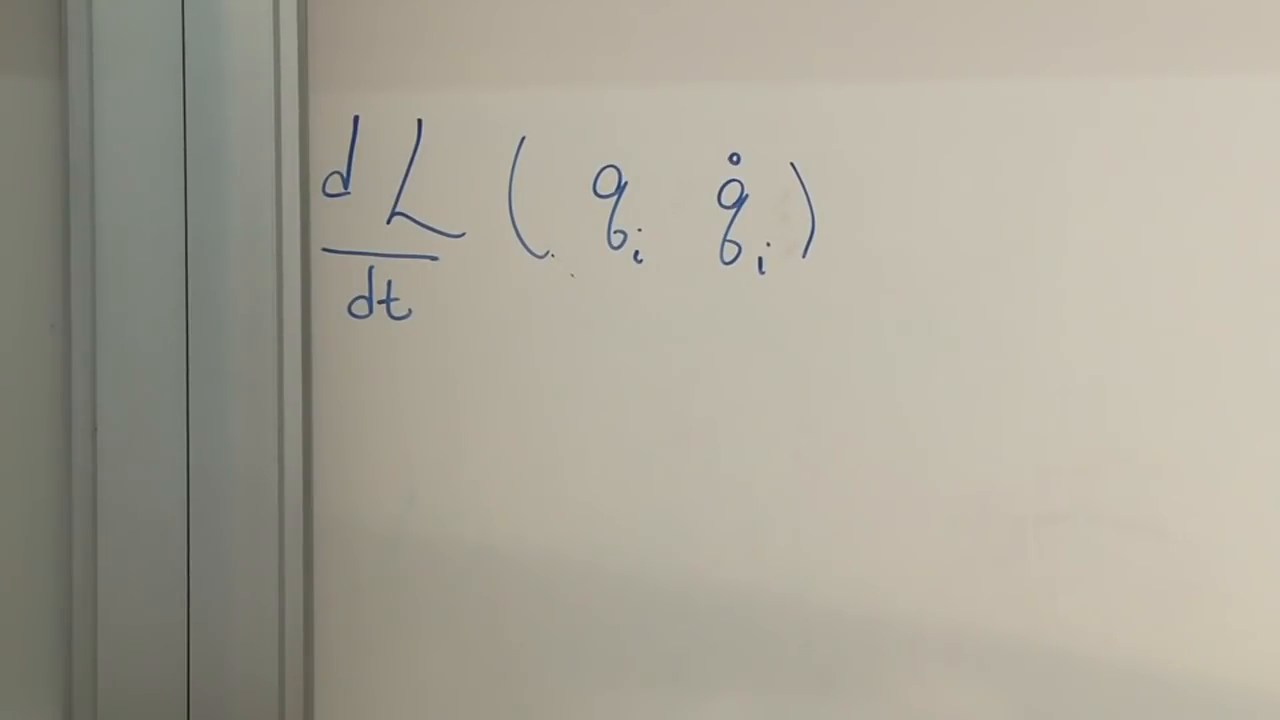
\includegraphics[width=0.72\textwidth]{lecture_05_figure_02.png}
  \caption{開始沿運動軌跡對\(L(q_i,\dot q_i)\)微分。}
  \lectureframe{01:08:51}
\end{figure}

\begin{classroomqa}
  \audiencequestion{鏈鎖律的表示式是不是漏了求和符號？
  \lecturetimestamp{01:10:39--01:11:05}}
  \lecturerresponse{是的。每個座標和每個速度都可能改變拉格朗日量，因此兩項都要對\(i\)求和。}
\end{classroomqa}

使用正則動量與尤拉--拉格朗日方程：
\begin{equation}
  p_i=\frac{\partial L}{\partial\dot q_i},
  \qquad
  \dot p_i=\frac{\partial L}{\partial q_i}.
  \label{eq:l5-p-and-pdot}
\end{equation}
於是式~\eqref{eq:l5-chain-rule-no-time}可寫成
\begin{align}
  \frac{dL}{dt}
  &=\sum_i(\dot p_i\dot q_i+p_i\ddot q_i)
  \notag\\
  &=\frac{d}{dt}\sum_i p_i\dot q_i.
  \label{eq:l5-product-rule}
\end{align}
其中的``巧妙之處''只是乘法法則。

\begin{figure}[htbp]
  \centering
  \includegraphics[width=0.84\textwidth]{lecture_05_figure_21.png}
  \caption{運用運動方程後，鏈鎖律便可改寫為\(\sum_i p_i\dot q_i\)的導數。}
  \lectureframe{01:13:45}
\end{figure}

\begin{classroomqa}
  \audiencequestion{乘積中的最後一個\(q_i\)應該帶一個點，還是兩個點？
  \lecturetimestamp{01:14:31--01:15:32}}
  \lecturerresponse{在乘積中，它是\(p_i\dot q_i\)，只帶一個點。對整個乘積微分會得到
  \(\dot p_i\dot q_i+p_i\ddot q_i\)，所以展開後第二項會出現兩個點。}
\end{classroomqa}

將這兩個導數相減，就得到一個守恆組合。依照歷史慣例，取其負值並稱為哈密頓量：
\begin{equation}
  H=\sum_i p_i\dot q_i-L.
  \label{eq:l5-hamiltonian-definition}
\end{equation}

\begin{figure}[htbp]
  \centering
  \includegraphics[width=0.80\textwidth]{lecture_05_figure_22.png}
  \caption{守恆組合\(L-\sum_i p_i\dot q_i=-H\)與哈密頓量的定義。}
  \lectureframe{01:18:05}
\end{figure}

對於處於勢中的單一粒子，
\begin{equation}
  L=\frac12m\dot x^2-V(x),
  \qquad p=m\dot x.
  \label{eq:l5-particle-lagrangian}
\end{equation}
因此
\begin{align}
  H&=p\dot x-L
  \notag\\
   &=m\dot x^2-\left(\frac12m\dot x^2-V(x)\right)
  \notag\\
   &=\frac12m\dot x^2+V(x)=T+V.
  \label{eq:l5-particle-energy}
\end{align}

\begin{figure}[htbp]
  \centering
  \includegraphics[width=0.86\textwidth]{lecture_05_figure_23.png}
  \caption{處於勢中的粒子，其哈密頓量化為熟悉的動能加勢能。}
  \lectureframe{01:20:50}
\end{figure}

推導過程沒有假設\(L\)必須具有特定形式。因此，在這套形式架構中，能量的一般定義是式~\eqref{eq:l5-hamiltonian-definition}，而不是\(T+V\)。

\section{顯式時間依賴與能量交換}

在鏈鎖律中加入顯式時間依賴：
\begin{equation}
  \frac{dL}{dt}
  =\sum_i\left(
    \frac{\partial L}{\partial q_i}\dot q_i
    +\frac{\partial L}{\partial\dot q_i}\ddot q_i
  \right)
  +\frac{\partial L}{\partial t}.
  \label{eq:l5-full-chain-rule}
\end{equation}
左側是沿著運動軌跡取的全導數。最後的偏導數在\(q\)與\(\dot q\)固定時取值，只對隨外部變化的參數微分。重做同樣的乘法法則步驟，可得
\begin{equation}
  \boxed{\frac{dH}{dt}=-\frac{\partial L}{\partial t}}.
  \label{eq:l5-hamiltonian-time}
\end{equation}

\begin{figure}[htbp]
  \centering
  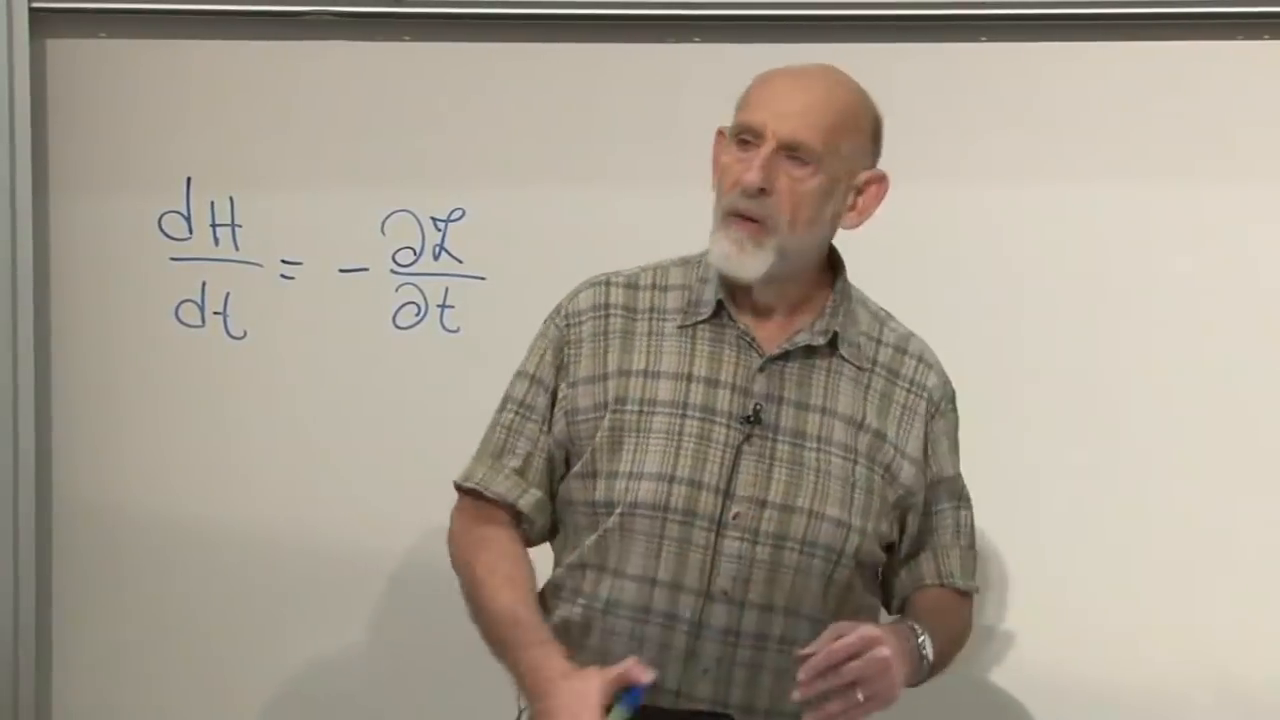
\includegraphics[width=0.70\textwidth]{lecture_05_figure_04.png}
  \caption{哈密頓量的變化只來自拉格朗日量的顯式時間依賴。}
  \lectureframe{01:37:22}
\end{figure}

對於式~\eqref{eq:l5-driven-oscillator}所示的受驅振子，
\begin{equation}
  \frac{\partial L}{\partial t}
  =-\frac12\dot k(t)x^2,
  \qquad
  \dot H=\frac12\dot k(t)x^2.
  \label{eq:l5-driven-energy-rate}
\end{equation}
在\(x=0\)處，瞬時變化率為零；在離開原點的位置，改變彈簧常數所作功的速率正比於\(x^2\dot k\)。

\begin{classroomqa}
  \audiencequestion{若能量不守恆，它的定義是否就是哈密頓量的時間導數？
  \lecturetimestamp{01:27:11--01:28:04}}
  \lecturerresponse{不是。能量就是\(H\)；它的導數則描述能量如何變化。拉格朗日量具有熟悉形式時，\(H=T+V\)；若不是，則由式~\eqref{eq:l5-hamiltonian-definition}定義。將外部驅動器也納入系統後，總哈密頓量便恢復守恆。}
\end{classroomqa}

\begin{classroomqa}
  \audiencequestion{這如何應用到先前那個旋轉木馬上的觀察者？當時出現了離心項與科里奧利項。
  \lecturetimestamp{01:28:08--01:29:52}}
  \lecturerresponse{勻速旋轉的座標系涉及隨時間變化的變數轉換，並非固定的空間對稱性，也不是單純的時間平移。可以從轉換後的拉格朗日量構造哈密頓量，但最好等到討論磁力時再進行這項獨立計算，因為兩者的代數形式十分相近。}
\end{classroomqa}

\section{拉格朗日力學工具一覽}

現在可以將整個架構簡潔地整理如下：
\begin{align}
  L&=L(q_i,\dot q_i,t),
  \notag\\
  p_i&=\frac{\partial L}{\partial\dot q_i},
  \qquad
  \dot p_i=\frac{\partial L}{\partial q_i},
  \notag\\
  \delta q_i&=\epsilon f_i(q)
  \quad\Longrightarrow\quad
  Q=\sum_i p_i f_i(q),\quad \dot Q=0,
  \notag\\
  H&=\sum_i p_i\dot q_i-L,
  \qquad
  \dot H=-\frac{\partial L}{\partial t}.
  \label{eq:l5-toolkit}
\end{align}

\begin{figure}[htbp]
  \centering
  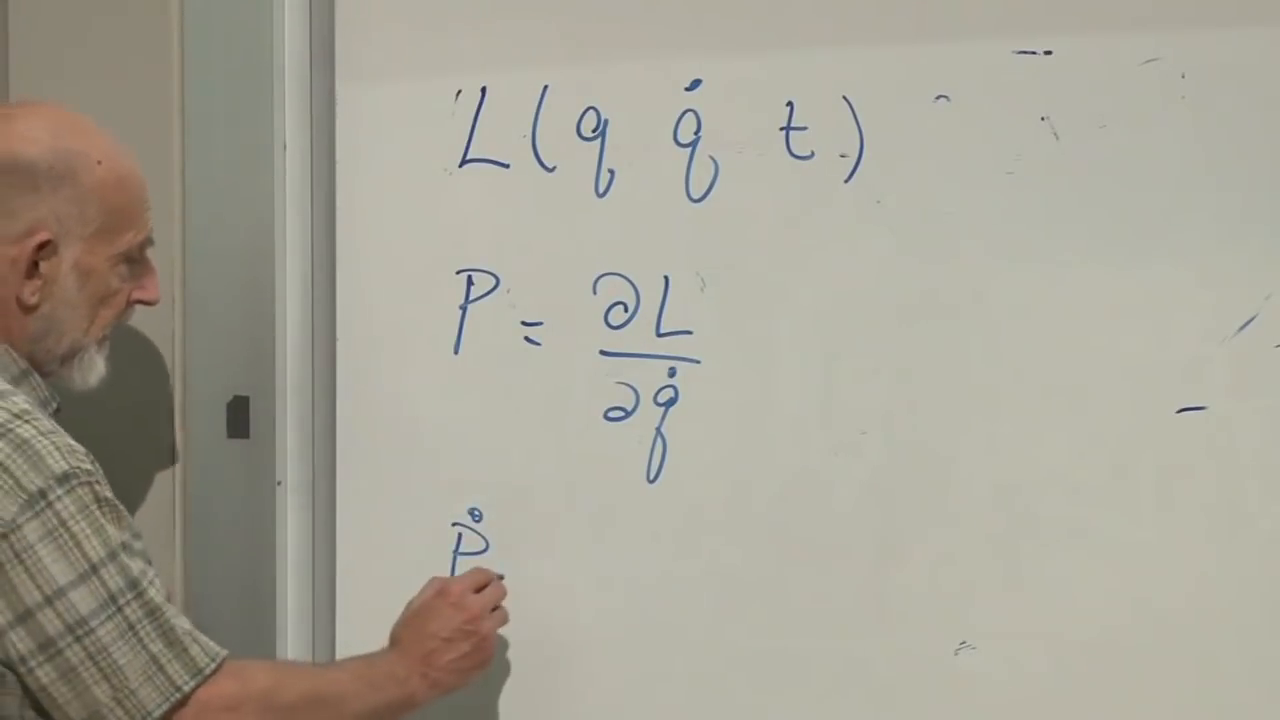
\includegraphics[width=0.66\textwidth]{lecture_05_figure_03.png}
  \caption{板書回顧從\(L(q,\dot q,t)\)、正則動量與尤拉--拉格朗日方程開始。}
  \lectureframe{01:31:37}
\end{figure}

這些公式涵蓋了定義、運動方程、一般連續對稱性所對應的守恆量，以及時間平移所對應的守恆量。需要記住的技巧不多；重要的是能重新推導這些公式，而不是死記彼此無關的表示式。

\section{為什麼要使用拉格朗日力學或哈密頓力學？}

\begin{classroomqa}
  \audiencequestion{力學是否可以同樣用\(L\)或\(H\)來描述？為什麼要選擇其中一種表述？
  \lecturetimestamp{01:37:16--01:39:18}}
  \lecturerresponse{只要勒讓德變換是正則的，兩種表述便等價，但它們著重的結構不同。拉格朗日力學自然地從作用量取駐值出發。哈密頓力學一開始較抽象，但其方程簡潔，且在量子力學中居於核心地位。哈密頓量雖然就是能量，其作用遠不止表達能量守恆。}
\end{classroomqa}

\begin{classroomqa}
  \audiencequestion{牛頓知道能量守恆的哈密頓形式嗎？
  \lecturetimestamp{01:39:29--01:39:56}}
  \lecturerresponse{就歷史記錄所示，牛頓並未使用這種表述。他提出的架構是力定律\(F=ma\)。}
\end{classroomqa}

\begin{classroomqa}
  \audiencequestion{為什麼每個物理系統都應該有拉格朗日量？這只是實驗上的事實嗎？
  \lecturetimestamp{01:39:57--01:42:37}}
  \lecturerresponse{對於此處討論的封閉系統，這是經驗事實，也能從更深層的量子描述導出。數學上自洽、但不是尤拉--拉格朗日方程的微分方程，可以人為構造出來。例如，\(\dot x=-x\)完全可以求解；但若把它當作描述封閉系統的基本單座標定律，它就具有耗散系統那種資訊流失的特徵。經典力學在邏輯上並不先於量子力學；它的基本架構承襲自量子力學。詳細原因留待後續說明。}
\end{classroomqa}

\begin{classroomqa}
  \audiencequestion{如果每個真實的封閉系統都有拉格朗日量，那麼我們稱作拉格朗日量的每個函數，都對應於自然界中實際存在的系統嗎？
  \lecturetimestamp{01:42:39--01:42:54}}
  \lecturerresponse{不是。形式演算容許許多函數，但目前已知的物理系統並未實現其中許多函數。}
\end{classroomqa}

\begin{classroomqa}
  \audiencequestion{拉格朗日量主要是用來發明勢能的工具嗎？
  \lecturetimestamp{01:42:54--01:43:32}}
  \lecturerresponse{它的用途更廣。它可以用來整理可能的力學系統，而且常是導出運動方程最簡便實用的方法。}
\end{classroomqa}

雙擺展現了這種實用上的優勢。選定兩個角度，依據這兩個角度及其時間導數，計算兩個質量的速度，再構造\(T-V\)，讓尤拉--拉格朗日方程以隱含方式處理約束力。這比用\(F=ma\)逐一求解所有張力與加速度，簡潔得多。

\begin{figure}[htbp]
  \centering
  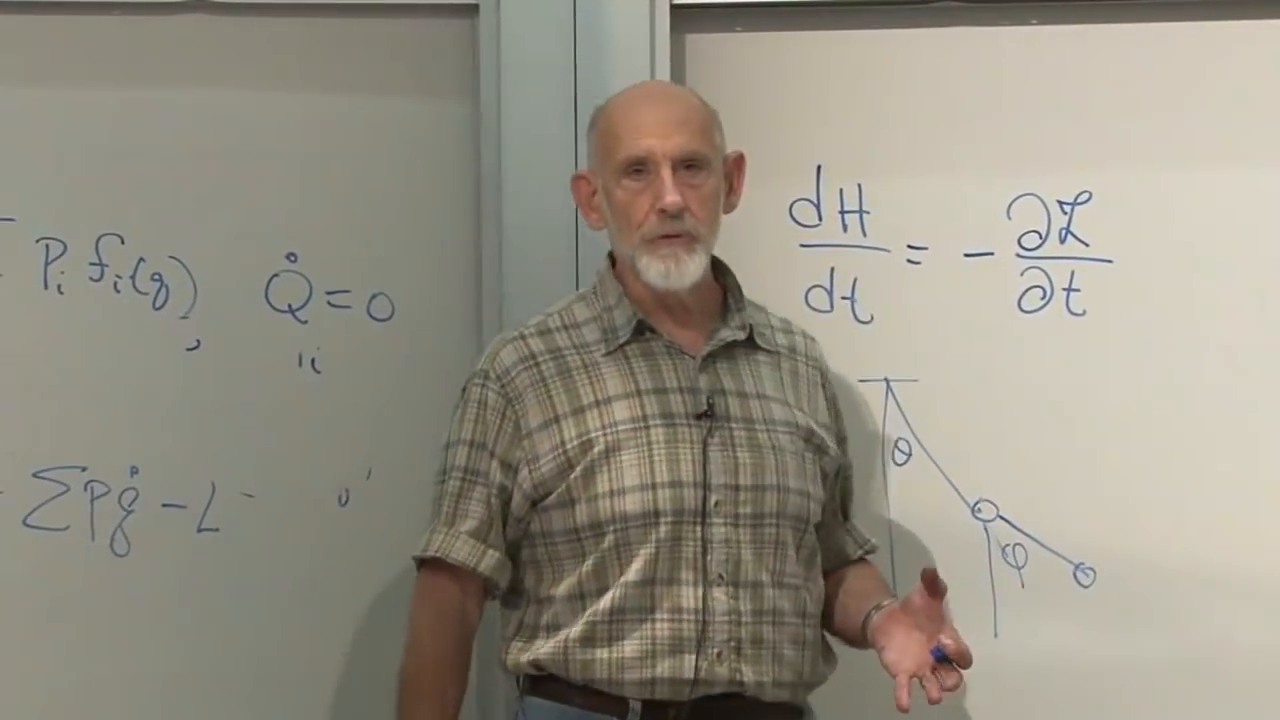
\includegraphics[width=0.84\textwidth]{lecture_05_figure_05.png}
  \caption{能量變化率的恆等式仍寫在黑板上，旁邊是雙擺示意圖。}
  \lectureframe{01:45:39}
\end{figure}

\begin{figure}[htbp]
  \centering
  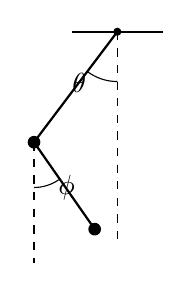
\begin{tikzpicture}[scale=1.15]
    \draw[thick] (-0.5,0) -- (0.5,0);
    \fill (0,0) circle (0.045);
    \draw[dashed] (0,0) -- (0,-2.3);
    \draw[thick] (0,0) -- (-0.92,-1.22);
    \fill (-0.92,-1.22) circle (0.07);
    \draw[dashed] (-0.92,-1.22) -- (-0.92,-2.55);
    \draw[thick] (-0.92,-1.22) -- (-0.25,-2.18);
    \fill (-0.25,-2.18) circle (0.07);
    \draw (0,-0.55) arc (-90:-127:0.55);
    \node at (-0.42,-0.56) {$\theta$};
    \draw (-0.92,-1.72) arc (-90:-55:0.48);
    \node at (-0.56,-1.72) {$\phi$};
  \end{tikzpicture}
  \caption{雙擺的廣義角座標。}
\end{figure}

變數轉換同樣有效率：先轉換拉格朗日量，再由它導出運動方程，不必分別轉換每一條力方程。

\begin{classroomqa}
  \audiencequestion{雙擺本質上是否也是另一個三體系統，例如太陽、地球和月球，只是把其中一個物體視為錨定物？
  \lecturetimestamp{01:45:06--01:45:25}}
  \lecturerresponse{這個類比點出了兩者的層級關係，雖然桿件施加的是不同約束。在這兩種情況下，都可以在近似中把質量極大或固定的組成部分視為參考結構。}
\end{classroomqa}

\begin{classroomqa}
  \audiencequestion{雙擺採用的是\(T-V\)，但剛才才強調過更一般的拉格朗日量。\(T-V\)在什麼情況下適用？
  \lecturetimestamp{01:46:08--01:46:58}}
  \lecturerresponse{對於在慣性參考系中觀察、且沒有磁性速度耦合的普通非相對論性粒子，這個熟悉的形式適用。旋轉參考系、相對論系統和磁場則需要更一般的項。}
\end{classroomqa}

\begin{classroomqa}
  \audiencequestion{碰撞不屬於這種描述嗎？
  \lecturetimestamp{01:47:00--01:48:05}}
  \lecturerresponse{彈性碰撞源於短程力，因此也可由勢能描述。非彈性碰撞在微觀層次上仍屬於力學現象，但能量會進入內部振動、形變和熱。若質心描述忽略了這些自由度，就不完整。}
\end{classroomqa}

\begin{classroomqa}
  \audiencequestion{棒球被球棒擊中時，可以用\(F=ma\)來分析嗎？
  \lecturetimestamp{01:48:05--01:48:33}}
  \lecturerresponse{只能在粗略的層次上分析。完整的描述必須追蹤形變、升溫、球可能受到的損傷，甚至球棒是否折斷。正因為有這些內部自由度，真實的撞擊才比質點碰撞複雜得多。}
\end{classroomqa}

\begin{classroomqa}
  \audiencequestion{那麼延展的剛體呢？
  \lecturetimestamp{01:48:34--01:49:00}}
  \lecturerresponse{研究剛體可以採用牛頓力學方法，也可以用以平動與轉動座標表示的\(T-V\)拉格朗日量。建構這個拉格朗日量是很好的練習。}
\end{classroomqa}

\begin{classroomqa}
  \audiencequestion{量子力學中的能量--時間不確定性關係，是否意味著能量不會嚴格守恆？
  \lecturetimestamp{01:49:01--01:49:29}}
  \lecturerresponse{不會。能量可以嚴格守恆。這個關係表示，要高精度地測定能量，需要長時間觀測；它並不取代守恆定律。}
\end{classroomqa}

\begin{classroomqa}
  \audiencequestion{牛頓力學與拉格朗日力學在邏輯上等價嗎？
  \lecturetimestamp{01:49:36--01:50:07}}
  \lecturerresponse{在兩種表述都適用的一般範圍內，它們是等價的。不過，也可以構造出某些拉格朗日量，使其方程不像基本形式\(m\ddot x=F(x)\)。}
\end{classroomqa}

\section{座標依賴的動能項}

考慮下面這個刻意選得較不尋常的例子
\begin{equation}
  L=\frac12q^2\dot q^2-\frac12q^2.
  \label{eq:l5-nonstandard-l}
\end{equation}
這是一個有效的拉格朗日量，其中的動能係數依賴座標。也可以考慮速度的一次項，例如\(q\dot q\)；在這個一維例子中，這個特定項是全導數，因此不會改變運動方程。

正則動量為
\begin{equation}
  p=\frac{\partial L}{\partial\dot q}=q^2\dot q,
  \label{eq:l5-nonstandard-p}
\end{equation}
因此
\begin{equation}
  \dot p=q^2\ddot q+2q\dot q^2,
  \qquad
  \frac{\partial L}{\partial q}=q\dot q^2-q.
  \label{eq:l5-nonstandard-derivatives}
\end{equation}
運動方程便是
\begin{equation}
  q^2\ddot q+q\dot q^2=-q.
  \label{eq:l5-nonstandard-eom}
\end{equation}

\begin{figure}[htbp]
  \centering
  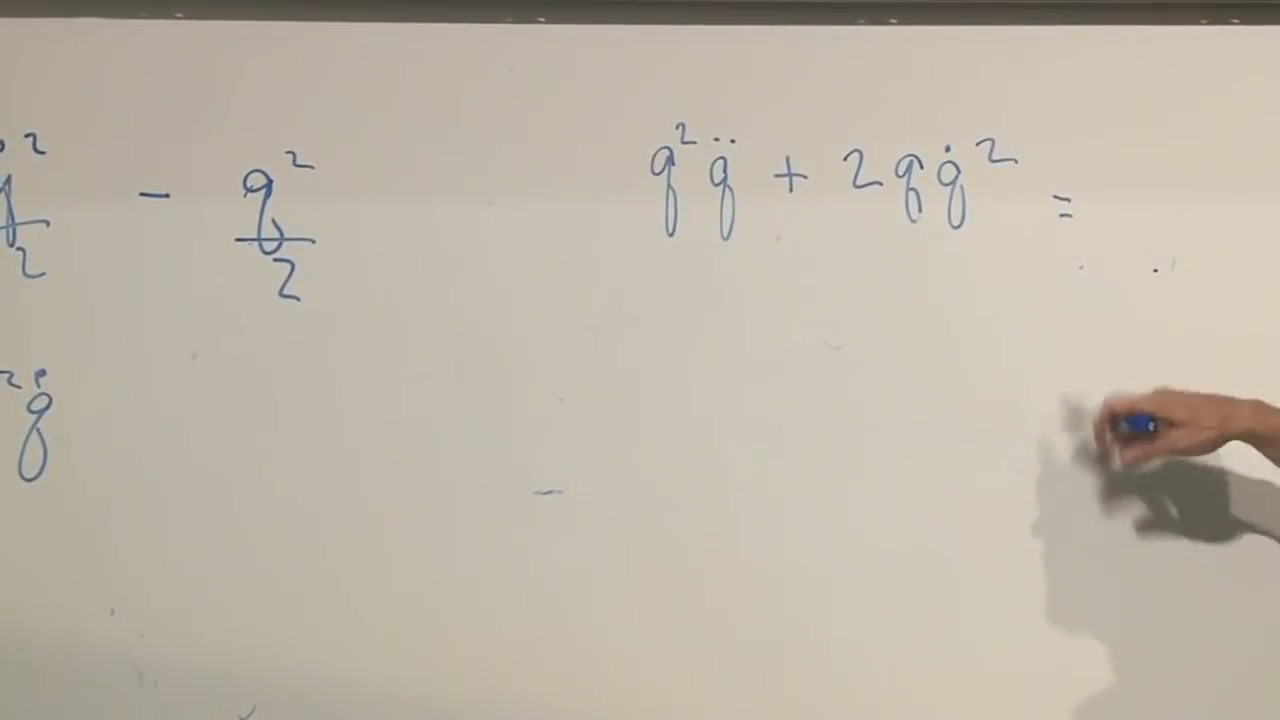
\includegraphics[width=0.80\textwidth]{lecture_05_figure_06.png}
  \caption{座標依賴動能例子中，對動量求導所得的結果。}
  \lectureframe{01:52:32}
\end{figure}

\begin{classroomqa}
  \audiencequestion{可以把方程兩邊除以\(q\)嗎？
  \lecturetimestamp{01:53:22--01:53:39}}
  \lecturerresponse{只有在\(q\neq0\)時才可以。在\(q=0\)時，動能係數與勒讓德映射會退化；若直接相除，就會略過這個必須另行處理的奇異點。}
\end{classroomqa}

哈密頓量為
\begin{align}
  H&=p\dot q-L
  \notag\\
   &=q^2\dot q^2-
     \left(\frac12q^2\dot q^2-\frac12q^2\right)
  \notag\\
   &=\frac12q^2\dot q^2+\frac12q^2.
  \label{eq:l5-nonstandard-h}
\end{align}

\begin{classroomqa}
  \audiencequestion{\(q^2\dot q^2/2\)仍然可以稱為動能嗎？
  \lecturetimestamp{01:54:41--01:55:07}}
  \lecturerresponse{可以。在這個例子中，哈密頓量再次呈現為正的動能項加上勢能項。這裡的重點是，即使事先不假設基本的常質量形式，這些形式定義仍然適用。}
\end{classroomqa}

\section{耗散與形式體系更深層的起源}

\begin{classroomqa}
  \audiencequestion{如何將摩擦納入拉格朗日量？
  \lecturetimestamp{01:55:09--01:56:17}}
  \lecturerresponse{在這裡討論的簡單、封閉且自由度有限的系統中，摩擦並不是以基本力的形式納入的。宏觀摩擦是大量微觀自由度所造成的統計效應。那些原子仍然遵循底層力學，但若約化描述不追蹤它們，就會呈現出耗散。}
\end{classroomqa}

\begin{classroomqa}
  \audiencequestion{哈密頓是如何得出他的表述的？
  \lecturetimestamp{01:56:22--01:56:37}}
  \lecturerresponse{這裡沒有介紹歷史上的推導。對本課程而言，重要的是理解這種表述如何運作。}
\end{classroomqa}

\begin{classroomqa}
  \audiencequestion{若拉格朗日量不明顯地具有\(T-V\)的形式，有沒有更一般的方法可以求得它？
  \lecturetimestamp{01:56:43--01:58:54}}
  \lecturerresponse{實驗、有根據的猜測、對稱性原理，或從期望的方程反推，都可以用來找出這個函數。問微積分本身它的輸入從何而來，就像問導數定義中的\(f(x)\)從何而來一樣。函數一旦指定，微積分就會告訴我們該怎麼做。至於自然界的封閉系統為何符合這種抽象結構，量子力學會從更深的層次給出答案。}
\end{classroomqa}

這一點與本課程開頭談到的主題相連。基本的哈密頓演化具有決定性且可逆；也就是說，軌跡不會合併，資訊也不會就此消失。這項性質與相空間表述的關係，將分階段展開。

\begin{classroomqa}
  \audiencequestion{變分法是否只是從預期的經典方程反向推導而來？量子力學也是用同樣的方法求得拉格朗日量嗎？
  \lecturetimestamp{01:59:37--02:01:07}}
  \lecturerresponse{在初等的經典力學建構中，確實可以選擇一個作用量，使作用量取駐值的路徑重現已知方程。量子力學的邏輯順序則不同：它自然地從哈密頓量出發，再進一步導出拉格朗日描述。哈密頓量在量子力學中更為直觀，雖然它在經典力學中初看之下較為抽象。}
\end{classroomqa}

\begin{classroomqa}
  \audiencequestion{量子力學能描述摩擦嗎？
  \lecturetimestamp{02:01:08--02:02:05}}
  \lecturerresponse{可以，但基本描述必須納入環境的自由度。若不考慮流體中的粒子，就無法完整描述在黏性流體中運動的粒子。當這些自由度沒有逐一追蹤時，摩擦便是隨之湧現的複雜集體效應。}
\end{classroomqa}
